%Du begynder bare at skrive
\chapter{Speciel Relativitetsteori}

Tilbage i 1905 præsenterede Albert Einstein første del af hvad, der i daglig tale kaldes for relativitetsteorien. Teorien beskæftiger sig med objekter i bevægelse og forudsiger effekter, som har været helt ukendte i den klassiske mekanik, og som for mange strider mod al logik. Tid er relativt, længder kan ændre sig, masse og energi er det samme og lysets hastighed i vakuum kan aldrig overskrides. Alt dette er blevet kendt som Einsteins specielle relativitetsteori, og vil i dette kapitel blive gennemgået. I vil komme forbi de generelle principper og ligninger, der danner grundlaget for teorien, og I vil komme til at beskæftige jer med nogle af de fascinerende konsekvenser, teorien har. Den anden del, fremlagt i 1916, er kendt som den almene (eller generelle) relativitetsteori. Den er en beskrivelse af tyngdekraft, og mindst lige så spændende. Den er dog også matematisk set langt mere kompleks, og vi vil derfor ikke dække det i løbet af ugen.

\section{Reference-- og Inertialsystemer}

Idéen om relativitet er ikke noget nyt koncept. Princippet blev første gang formuleret af Galileo Galilei i 1630, og mange har siden beskæftiget sig med det, deriblandt Isaac Newton. Inden vi går igang med at undersøge Einsteins relativitetsprincip, må vi først stifte et bekendtskab med Galileis og Newtons arbejde inden for emnet. For at kunne gøre dette, skal vi dog først have styr på begreberne \textit{referencesystem} og \textit{inertialsystem}.

Når man anvender fysiske love, fastlægger man oftest et koordinatsystem, i forhold til hvilket man kan bestemme fysiske størrelser såsom position, hastighed, acceleration og lignende. Da man ikke kan måle en partikels position med hensyn til et abstrakt matematisk punkt, men kun ud fra et fysisk legeme, kan et koordinatsystem kun fastlægges ved at referere til et fysisk legeme. Et sådan  referencelegeme og det tilsvarende koordinatsystem kaldes for et \textit{referencesystem}. Der forudsættes her, at rummets geometri er Euklidisk, det vil sige at rummet ikke "krummer", og Pythagoras sætning er gældende. Herudover må tiden, \textit{t}, være defineret i hele rummet, da det indgår i de fysiske love. I den Galileiske og Newtonske relativitetsteori er tiden absolut og tikker af sted med samme rate overalt i universet. Det er her kun valget af enheder og nulpunkt, der frit kan vælges i et referencesystem. 

Et referencesystem, hvori Newtons første lov er gældende, kaldes et \textit{inertialsystem}. Med dette menes der referencesystemer, som bevæger sig med en jævn (konstant) hastighed og ikke foretager nogle accelererede bevægelser. Sådanne systemmer foretrækkes ofte, da alle Newtons love gør sig gældende i dem. 

I praksis er det dog vanskeligt at finde nogle perfekte inertialsystemer i vores verden. Hvis vi f.eks. placerer et referencesystem på Jorden, bliver vi nød til at tage Jordens rotation i betragtning. Referencesystemet roterer altså, og er dermed ikke et inertielt referencesystem, da det foretager en accelereret bevægelse. I sådanne ikke-inertielle referencesystemer vil frie partikler udføre accelererede bevægelser.

I det næste kapitel vil vi undersøge, hvordan man kan beskrive en begivenhed set fra forskellige inertialsystemer. Et eksempel på dette ville f.eks. være at betragte et lysglimt fra et tog, der bevæger sig med en hvis hastighed i forhold til togperronen.

\section{Galilei--Transformation}

\begin{figure}[h!]
	\centering
	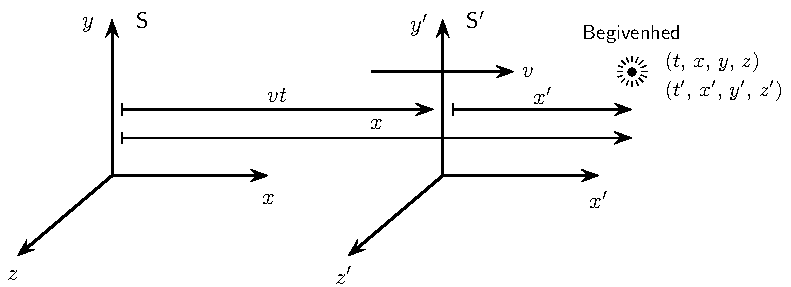
\includegraphics[scale=1]{Relativitetsteori/Galilei.pdf}
	\caption{$S$ og $S'$ i standardkonfiguration, med en begivenhed.}
	\label{sr.fig1}
\end{figure}

Før Einsteins revolutionerede forståelsen af relativitet var den gængse opfattelse den, der var udviklet af Galilei. Den bliver derfor kaldt for Galilieisk relativitet, og skønt vi ved, at den ikke er helt korrekt, så passer den stadig godt ved hastigheder langt mindre end lysets hastighed. 
Når man beskæftiger sig med relativitetsteori, er det meget vigtigt at anvende et præcist sprogbrug for at undgå misforståelser og fejl. Grundlæggende for en præcis beskrivelse af fysiske fænomener er begrebet en begivenhed. En begivenhed defineres som en øjeblikkelig hændelse, der sker i ét punkt, som f.eks. et lysglimt. Denne begivenhed er beskrevet ved koordinaterne $(x,y,z,t)$.
Lad os betragte to inertialsystemer $S$ og $S’$ i standard konfigurationen, som bevæger sig med en jævn, retlinjet hastighed v i forhold til hinanden. Standard konfigurationen er en særligt anvendelig måde at sammenligne to inertialsystemer på, og kan ses i Figur \ref{sr.fig1}. Når de to inertialsystemer er i standardkonfiguration, menes der, at de bevæger sig langs x-aksen med en hastighed \textit{v} med hensyn til hinanden, mens de resterende akser er parallele. Herudover er de to systemers nulpunkter sammenfaldende til tiden $$t=t'=0$$ Antager vi nu, at en begivenhed har koordinaterne $(t, x, y, z)$ i $S$ og $(t’, x’, y’, z’)$ i $S’$, så er forholdet mellem disse to koordinatsæt intuitivt givet ved Galilei-transformationen,


\begin{empheq}[box=\fbox]{align}
\begin{split}
&t'=t \\
	&x'=x-v\cdot t \\
	&y'=y \\
	&z'=z
	\end{split}
	\label{sr.eq1}
\end{empheq}

Her er $v$ hastigheden af $S’$ i forhold til $S$. Dette underbygges af at betragte Figur \ref{sr.fig1}, da afstanden mellem de to referencesystemers nulpunkter er $v\cdot t$.

Ved at differentiere venstresiderne af \ref{sr.eq1} med hensyn til $t’$ og højresiderne med hensyn til $t$, får vi de klassiske hastighedstransformationer, som giver en sammenhæng mellem hastigheden af en partikel i $S$ og $S’$,

\begin{empheq}[box=\fbox]{align}
\begin{split}
	&u'_x=u_x-v \\
	&u'_y=u_y \\
	&u'_z=u_z
\end{split}
\label{sr.eq2}
\end{empheq}

hvor $(u_x, u_y, u_z)=(dx/dt, dy/dt, dz/dt)$ og $(u'_x, u'_y, u'_z)=(dx'/dt', dy'/dt', dz'/dt')$. Sammensætningen af parallelle hastigheder foregår herved ved addition. Et eksempel på dette er hvis du bevæger dig langs et tog med 5 km/t ($u'_x$), og toget kører med 100 km/t (v), vil du bevæge dig med 105 km/t i forhold til sporet. Dette er dog ikke tilfældet i den specielle relativitetsteori.
Ved at differentiere endnu en gang, fås transformationsreglerne for accelerationen,

\begin{empheq}[box=\fbox]{align}
\begin{split}
&a'_x=a_x \\
&a'_y=a_y \\
&a'_z=a_z
\end{split}
\label{sr.eq3}
\end{empheq}

\section{Det Specielle Relativitetsprincip}

Omkring 1860 udgav James Clerk Maxwell sin berømte teori om elektromagnetismen, og i denne teori opstod en særlig konstant c med enheder som en hastighed. Hans teori forudsagde, blandt andet, at ændringer i det elektromagnetiske felt i vakuum udbreder sig med denne hastighed c. Med andre ord, så forudsagde den eksistensen af elektromagnetiske bølger. Det overraskende her var, at hastigheden c tilfældigvis var sammenfaldende med lysets hastighed (bestemt ved forsøg), og førte til Maxwells konklusion om, at lys består af elektromagnetiske bølger. Som bærer af disse bølger, genoplivede Maxwell den gamle æterteori, en teori benyttet af Newton i sin tid til at beskrive udbredelsen af lys i form af bølger. Denne teori krævede et medie, æteren, for at lyset kunne udbrede sig som bølger, analog til lydbølger der udbreder sig i luften. Herudfra fortolkede han hastigheden c som udbredelseshastigheden af elektromagnetiske bølger i forhold til æteren. Det var herved muligt at definere et særligt absolut inertialsystem, nemlig det der var i i hvile i forhold til æteren, som kunne være Newtons absolutte rum. 

Æteren blev således et centralt emne for studie og debat i slutningen af det 19. århundrede. Man søgte i særdeleshed at fastlægge hastigheden af Jordens bevægelse gennem æteren, ved at måle den såkaldte ”æter-vind”. Princippet i disse forsøg var, at lysets hastighed ville variere, eftersom lysstrålen bevægede sig med eller mod Jordens bevægelse i forhold til æteren. Ingen ændring i lysets hastighed blev observeret i løbet af det halve år som forsøget varede. Den mest åbenbare forklaring på dette ville være, at Jorden ikke bevægede sig i forhold til æteren, eller med andre ord, at æteren tog del i Jordens bevægelse ligesom atmosfæren. Der opstod dog vanskeligheder med denne forklaring, idet man ikke kunne tænke sig, at Jorden under sin bevægelse medførte æteren overalt i verdensrummet. Dette efterlod den elektromagnetiske teori med et paradoks: Lysets gennemsnitlige hastighed for en frem-og-tilbage-rejse var uafhængig af ætervinden.
Einsteins forklaring på ætervinds-paradokset var drastisk, sammenlignet med andre forsøg. Med henvisning til den klassiske mekaniks relativitetsprincip, fremsatte han i 1905 sit berømte specielle relativitetsprincip, hvis første postulat er

\begin{framed}
	\centering
	Alle intertialsystemer er ligeværdige for udførelsen af alle fysiske eksperimenter
\end{framed}

Ifølge dette postulat findes der herved ingen æter, og dermed intet absolut rum. Alle inertialsystemer er fuldstændige ligeværdige, da samtlige fysiske love gælder uforandret i dem alle. I særdeleshed gælder de samme elektromagnetiske og optiske love, som førte Einstein til sit andet postulat,

\begin{framed}
	\centering
	I det tomme rum udbreder lyset sig retlinjet med hastigheden $c$ i enhver retning i ethvert inertialsystem.
\end{framed}

Hvad dette postulat betyder, er at lige meget hvor hurtigt man forfølger en lysstråle (ved at forflytte sig til hurtigere inertialsystemer), vil man se lysstrålen udbrede sig med hastigheden c. Einsteins store bedrift var, at han var i stand til at finde en ny struktur for rum og tid, der kunne imødekomme begge disse postulater. Dette krævede en udskiftning af Galilei-transformationen som den grundlæggende forbindelse mellem inertialsystemer. Denne nye transformation, Lorentz-transformationen, krævede indførelsen af begrebet relativ tid, som ikke adskiller sig fra den absolutte tid i det enkelte inertialsystem, men som er forskellig fra system til system. Vi vil se nærmere på dette i det næste kapitel, ved hjælp af et af Einsteins berømte tankeeksperimenter.

\section{Samtidighed}

Vi tænker os to inertialsystemer, $S$ og $S’$, med hver sine tidsmål $t$ og $t’$. I den klassiske mekanik går man ud fra at disse to tidsmål stemmer overens, og i Galilie-transformationen sætter man derfor $t = t’$. Dette kan man ikke uden videre opretholde i relativitetsteorien. Derfor søger vi en definition for samtidighed, der tillader os at afgøre om to begivenheder er samtidige eller ikke ud fra fysiske målinger. Ved at benytte os af Einsteins andet postulat, kan vi indføre den følgende definition for samtidighed, 

\begin{framed}
	\centering
	To begivenheder, der foregår i punkterne A og B, siges at være samtidige såfremt et lyssignal udsendt fra A, når begivenheden her finder sted, og et lyssignal udsendt fra B, når begivenheden finder sted der, vil nå frem til en iagttager i samme afstand fra A og B til samme tidspunkt.
\end{framed}

Denne definition medfører, at to iagttagere i indbyrdes bevægelse oftest ikke vil være enige om samtidigheden af to begivenheder.

\begin{figure}[h!]
	\centering
	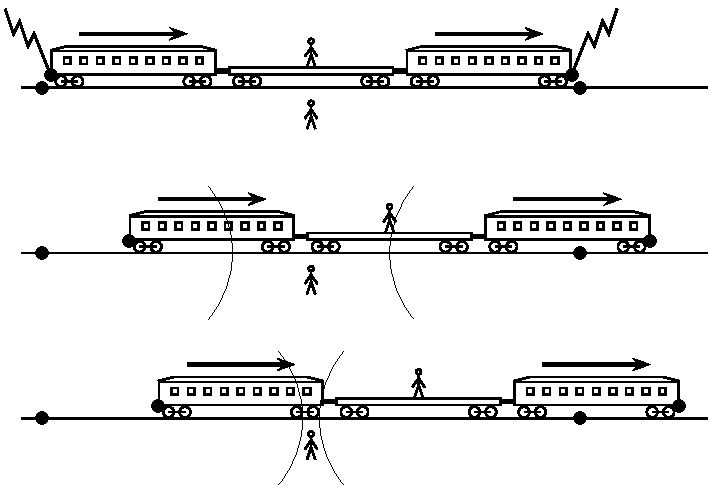
\includegraphics[scale=1]{Relativitetsteori/Tog.pdf}
	\caption{Einsteins berømte tankeeksperiment.}
	\label{sr.tog}
\end{figure}

Einstein demonstrerede dette igennem det følgende berømte tankeeksperiment. Lad os betragte et tog i jævn retlinjet bevægelse i forhold til jordoverfladen, som antages at udgøre et inertialsystem. Herved udgør jordoverfladen et andet inertialsystem. Under et tordenvejr, slår et lyn ned ved togets forende og et andet ved togets bagende, således at der afsættes mærker på både toget og skinnerne. Herudover vil et lysglimt bevæge sig forlæns og baglæns langs toget, se Figur \ref{sr.tog}. En iagttager der befinder sig på jorden modtager de to lysglimt samtidig og, ved en måling af mærkerne på skinnerne, finder at han befandt sig midt imellem de to mærker. Herudfra må iagttageren konkludere, at de to begivenheder var samtidige ud fra vores definition.

Det interessante spørgsmål her, er om en iagttager der befandt sig på midten af toget ville komme til den samme konklusion. Set fra iagttageren på Jorden bevæger toget sig hen mod lysglimtet fra forenden og væk fra lysglimtet fra bagenden. Herved modtager iagttageren på toget lysglimtet fra forenden før lysglimtet fra bagenden. Denne iagttager kan efterfølgende måle sig frem til, at han/hun befinder sig lige langt fra hvert lynnedslag baseret på mærkerne på toget, og må ud fra dette konkludere at de to begivenheder ikke var samtidige. Det forreste lynnedslag skete tidligere en det bagerste lynnedslag. Dette skyldes at lyset, grundet Einsteins andet postulat, også bevæger sig med samme hastighed i enhver retning i denne iagttagers inertialsystem.

Skete de to lynnedslag så samtidigt eller ikke? Det sære og vidunderlige ved dette er, at der ikke er noget entydigt svar på dette spørgsmål. Set fra jord-systemet skete de samtidigt, men fra tog-systemet var de ikke samtidige. Herved er samtidighed derved et relativt begreb. Kun i specielle tilfælde, såsom hvor to begivenheder sker i et punkt, vil samtidighed i et inertialsystem medføre samtidighed i et andet.

\section{Længde}


Hvis en iagttager ønsker at måle længden af en stang i hvile i forhold til sig selv, kan han/hun som i det klassiske tilfælde gøre dette ved at placere en målestok langs stangen og finde differencen af de to endepunkters koordinater. Er stangen i bevægelse i forhold til iagttageren, kan man dog ikke bruge denne metode. En længdemåling kan defineres som følgende

\begin{framed}
	\centering
	Ved længden af en stang, der bevæger sig i sin længderetning parallelt med en målestok, forstår vi afstanden mellem to mærker afsat på målestokken ud for stangens endepunkter til samme tidspunkt.
\end{framed}

Det vigtige her, er at mærkerne skal afsættes samtidigt i forhold til den iagttager, der foretager længdemålingen, og derved i hvile i forhold til målestokken. En anden iagttager som er i bevægelse i forhold til den første vil, som vi så i det tidligere tankeeksperiment, finde at de to mærker er afsat til forskellige tidspunker, og derved finde en anden værdi for længden.

I det tidligere tankeeksperiment, ville iagttageren på jorden kunne måle togets længde ved at måle afstanden mellem de to mærker på skinnerne, da de jo for ham blev afsat samtidigt. Da iagttageren på toget kom til den konklusion, at mærket ved forenden blev afsat før mærket på bagenden, er afstanden mellem mærkerne på skinnerne for ham/hende mindre end togets længde. En iagttager, for hvem en stang er i bevægelse, vil altså finde en mindre værdi for stangens længde, end en iagttager for hvem stangen er i hvile. Den største længde findes altså i stangens hvilesystem, og denne længde kaldes derfor for hvilelængden.

\section{Varighed}

Ud fra vores konklusioner omkring samtidighed i relativitetsteorien, er det næsten klart, at varigheden af en proces må bedømmes forskelligt af to iagttagere i forskellige bevægelsestilstande, da disse jo er uenige om samtidigheden af to begivenheder. Hvis vi forestiller os et lille stykke fyrværkeri der antændes, går der et lille tidsrum inden det eksploderer. Er fyrværkeriet i hvile i forhold til iagttageren, vil iagttageren måle en vis varighed for processen, som kaldes for egentiden. En iagttager i bevægelse i forhold til fyrværkeriet vil se antændelsen og eksplosionen i forskellige punkter af sit eget inertialsystem, og vil i almindelighed finde en anden varighed. Vi vil undersøge dette koncept nærmere, efter vi har udledt Lorentz-transformationen.

\section{Lorentz--Transformationen}

Da vi nu har gennemgået de mest væsentlige begreber, vil vi kunne gå i gang med at udlede Lorentz-transformationen. Ligesom i Galilei-transformationen skal Lorentz-transformationen knytte en begivenheds koordinater $(x,y,z,t)$ i et inertialsystem $S$ med dets koordinater $(x’,y’,z’,t’)$ i et inertialsystem $S’$. Vi antager her, at $S$ og $S’$ mærke er indrettet i standardkonfigurationen, som ses i Figur \ref{sr.fig1}. Opgaven her er altså, med udgangspunkt i det specielle relativitetsprincip, at bestemme sammenhængen mellem de to koordinatsæt, som kan skrives på formen

\begin{align}
	\begin{split}
	&t'=f_t(t, x, y, z, v) \\
	&x'=f_x(t, x, y, z, v) \\
	&y'=f_y(t, x, y, z, v) \\
	&z'=f_z(t, x, y, z, v) 
	\end{split}
\end{align}

hvor de fire funktioner udover at afhænge af de oprindelige koordinater, kan afhænge af den relative hastighed $v$ mellem $S$ og $S’$.

Da inertialsystemerne er i standardkonfigurationen, kan vi herved slutte, at for enhver begivenhed er

\begin{align}
	y'=y \ \ , \ \ z'=z \nonumber
\end{align}

Herved har vi bestemt to af transformationsligningerne i Lorentz-transformationen. Ydermere kan vi fjerne afhængigheden af $y$ og $z$ i de tilbageværende funktioner, da en afhængighed af disse ville bryde med rummets homogenitet.

Vi har nu to transformationsligninger tilbage, som tager formen

\begin{align}
	\begin{split}
	&t'=f_t(x, t, v) \\
	&x'=f_x(x, t, v) 
	\end{split}
\end{align}

Til sammenligning er Galilei-transformationen for disse to koordinater

\begin{align*}
	&t'=t \\
	&x'=x-vt
\end{align*}

Transformationen er lineær og ydermere homogen. Med homogen menes der, at $(t,x)=(0,0)$ medfører $(t’,x’)=(0,0)$. En homogen transformation indeholder herved ikke konstante led. Ud fra vores antagelse om at de to inertialsystemer er i standardkonfiguration, vil transformation 3.5 være homogen, da de to systemer er sammenfaldende til tiden $t=t'=0$. Vi vil i den følgende udledelse gå ud fra, at Lorentz-transformationen også er lineær. Hvis transformationen ikke var lineær, ville en jævn bevægelse kunne transformeres til en jævn accelereret bevægelse, hvilket ville bryde med vores antagelse om, at $S$ og $S'$ er inertialsystemer. Ved denne antagelse, kan de to resterende transformationsligninger skrives som

\begin{align}
	\begin{split}
	&t'=\kappa x+\sigma t \\
	&x'=\gamma x+\rho t
	\end{split}
	\label{sr.eq4}
\end{align}

hvor $\kappa$, $\sigma$, $\gamma$, og $\rho$ kan afhænge af hastigheden $v$, men er uafhængige af $t$ og $x$.

Vi vil nu udnytte, at vi kender den relative hastighed af de to systemer $S$ og $S’$. Da $S’$ bevæger sig med hastigheden $v$ i forhold til $S$, følger det, at $S$ bevæger sig med hastigheden $-v$ i forhold til $S’$. Vi kræver nu at begyndelsespunktet for $S’$, \textbf{O'} ($x'=0$), har hastigheden $v$ set fra $S$. Ved at sætte $x'=0$ ind i den anden ligning af \ref{sr.eq4}, samt ved at indsætte $x=v\cdot t$, får vi følgende,

\begin{align}
	0=\gamma v&t+\rho t \nonumber \\
	&\Downarrow \nonumber \\
	v=-&\rho / \gamma
\end{align}

Tilsvarende må \textbf{O} ($x=0$) have hastigheden $-v$ i forhold til $S'$. Ved at sætte $x=0$ i de to transformationsligninger og indsætte de resulterende udtryk i $x'=-vt'$, får vi

\begin{align}
	\sigma=\gamma
\end{align}

Ved at benytte de to tidligere omskrivninger, samt ved at skrive $\kappa$ på formen $\kappa=-\gamma \alpha v$, kan transformationsligningerne reduceres til følgende,

\begin{align}
	&t'=\gamma*(t-\alpha vx) \\
	&x'=\gamma*(x-vt)
\end{align}

Herved har vi $\gamma$ og $\alpha$ tilbage som de ukendte funktioner af $v$. For at kunne bestemme disse to ukendte funktioner, skal vi betragte en lyskilde, som til tiden $t=t'=0$ udsender et lysglimt fra et fælles begyndelsespunkt i $S$ og $S'$. Som følge af Einsteins andet postulat, må dette lysglimt udbrede sig sfærisk med hastigheden $c$ i både $S$ og $S'$. Med andre ord skal sfærens radius i de to inertialsystemer være henholdsvis $r=ct$ og $r'=ct'$. Der vil altså gælde følgende,

\begin{align}
	&x^2+y^2+z^2=c^2t^2 \\
	&x'^2+y'^2+z'^2=c^2t'^2 \label{sr.eq5}
\end{align}

hvor vi her har benyttet os af Pythagoras sætning i 3 dimensioner, til at bestemme sfærens radius i $S$ og $S’$. Vi må nu kræve, at Lorentz-transformationen opfylder begge disse to udtryk for lysglimtets udbredelse.

Ved at benytte vores transformationsligninger på \ref{sr.eq5}, får vi

\begin{align}
	(\gamma x-\gamma vt)^2+y^2+&z^2=c^2(\gamma t-\gamma \alpha vx)^2 \nonumber \\
	&\Downarrow \nonumber \\
	\gamma^2x^2+\gamma^2v^2t^2-2\gamma^2xvt+y^2+z^2&=c^2\gamma^2t^2+c^2\gamma^2\alpha^2v^2x^2-2c^2\gamma^2\alpha xvt
\end{align}

Vi søger nu at bestemme $\gamma$ og $\alpha$ således at denne ligning er i overensstemmelse med lysets udbredelse i $S$. Vi bemærker først at de to led, der indeholder produktet $xvt$ må gå ud med hinanden, hvorved vi har

\begin{align}
	\alpha=1/c^2
\end{align}

Vi kan herefter samle de to led der indeholder $x^2$ på venstre siden og benytte $\alpha$,

\begin{align}
	x^2(\gamma^2-\gamma^2v^2/c^2)+y^2+z^2=c^2\gamma^2t^2-\gamma^2v^2t^2 \label{sr.eq6}
\end{align}

For at \ref{sr.eq6} stemmer overens med 3.11, må vi kræve at $x$'s koefficient er 1,

\begin{align}
	\gamma^2-\gamma^2v^2/c^2 = 1 \nonumber
\end{align}

Vi har således at $\gamma$ er,

\begin{empheq}[box=\fbox]{align}
\gamma = \gamma(v) = \frac{1}{\sqrt{1-v^2/c^2}}
\label{sr.eq7}
\end{empheq}

Funktionen $\gamma(v)$ er den berømte Lorentz-faktor, som spiller en vigtigt rolle i relativitetsteorien. For en hastighed $|v|>0$ er $\gamma(v)$ altid større end 1, men for hastigheder $|v|<<c$ er denne størrelsesforskel meget lille. Lorentz-faktoren er en funktion af den relative hastighed, $v$, af de to inertialsystemer. Man burde derfor betegne den som $\gamma(v)$, men da denne notation kan virke ret tung at benytte, vil vi fremover benytte notationen $\gamma$.

Da vi nu har udledt udtrykken for de to ubekendte, $\alpha$ og $\gamma$, kan vi opstille Lorentz-transformationens endelige form:

\begin{empheq}[box=\fbox]{align}
\begin{split}
&t'=\gamma(t-vx/c^2), \\
&x'=\gamma(x-vt), \\
&y'=y, \\
&z'=z
\end{split}
\end{empheq}

Dette ligningssæt kan løses med hensyn til variablerne $x, y, z, t,$ hvorved vi finder den omvendte Lorentz-transformation:

\begin{empheq}[box=\fbox]{align}
\begin{split}
&t=\gamma(t'+vx'/c^2), \\
&x=\gamma(x'+vt'), \\
&y=y', \\
&z=z
\end{split}
\end{empheq}


\section{Relativistiske Effekter}

Som I har set i de tidligere afsnit og specielt i forbindelse med Lorentz-transformationerne, må man i den specielle relativitetsteori  give slip på mange af vores gamle og intuitive ideer, omkring hvad tid, længde, samtidighed og varighed egentligt er for nogle størrelser. I dette afsnit skal vi kigge nærmere på (og give en mere matematisk beskrivelse af) nogle af de relativistiske effekter, der illustrerer, hvordan varighed og længde er relative størrelser.\\

En hurtigt bemærkning er, at der er flere måder at undersøge disse relativistiske effekter på. En taktik er at kigge nærmere på Lorentz-transformationerne, men det får I selv lov til at prøve kræfter med i opgaverne. Her vil vi i stedet starte et andet sted, nemlig Einsteins to postulater, og ud fra disse og nogle tankeeksperimenter undersøge, hvordan varighed og længde behandles i den specielle relativitetsteori.\\ 

\noindent
\textbf{Tidsforlængelse}\\

Som I har set i afsnittet om varighed, vil den tid det tager en proces at udfolde sig afhænge af, hvilket referencesystem processen observeres fra.
For at undersøge dette fænomen nærmere, kan man opstille et tankeeksperiment, der involverer to forskellige referencesystemer $S$ og $S'$. Her vælges $S'$ til at være et referencesystem, der er i hvile på en togperron, og $S$ vælges til at være et referencesystem, der er i hvile i et tog, som passerrer perronen med en konstant fart $v$. Det næste man skal bruge i tankeeksperimentet, er det, der kaldes et lysur. Et lysur består af to parallelle spejle, der er placeret i en afstand $d$ fra hinanden, som det er vist på Figur \ref{tidfor}. Man kan definere et enkelt tik på lysuret, som den tid det tager en foton, der skydes afsted fra det nederste spejl og lodret opad, at bevæge sig frem og tilbage. Ideen med tankeeksperiment er da, at placere et lysur så det er i hvile i toget, og undersøge hvordan et enkelt tik på uret ser ud, når det observeres af en observatør på perronen og af en observatør i toget.\\

Set fra en observatør i toget er lysuret i hvile, og denne observatør ser altså fotonen bevæge sig lodret op og ned, som det er vist på Figur \ref{tidfor}. Da fotonen, ifølge Einsteins andet postulat, bevæger sig med farten $c$ set fra alle inertielle referencesystemer, konkluderer denne observatør, at egentiden, $\Delta t$, for et enkelt tik på lysuret må være givet som:

\begin{equation}
\Delta t = \frac{2d}{c}
\label{tid_tog}
\end{equation}

\vspace{2mm}

Set fra en observatør på perronen er lysuret i bevægelse (da det befinder sig i toget), og denne observatør ser altså ikke fotonen bevæge sig lodret op og ned, men i stedet for skråt opad og nedad i den retning som toget bevæger sig, som ses på Figur \ref{tidfor}. Fotonen vil, igen pr. Einsteins andet postulat, også for denne observatør bevæge sig med farten $c$. Denne observatør konkluderer derfor, at tiden for et enkelt tik på lysuret set fra perronen, $\Delta t'$, må være:

\begin{equation}
\Delta t' = \frac{2L}{c}
\label{tid_perron}
\end{equation} 

\vspace{2mm}  

\begin{figure}[h!]
	\centering
	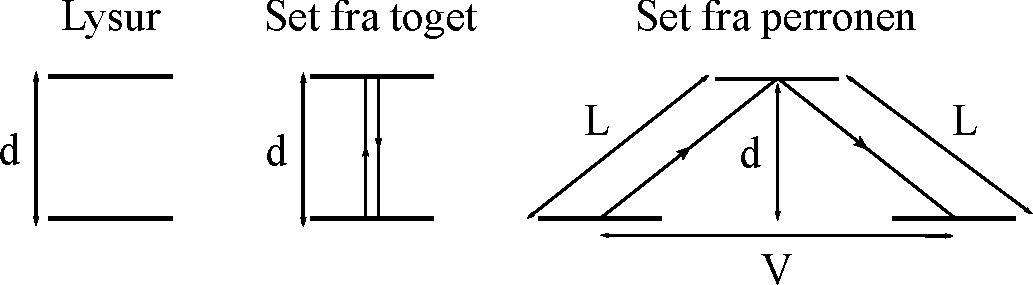
\includegraphics[scale=0.90]{Relativitetsteori/tidsforlang2.pdf}
	\caption{Til venstre i figuren ses et lysur. I midten ses et tik på lysuret set fra en observatør i toget. Til højre set et tik på lysuret set fra en observatør på perronen.}
	\label{tidfor}
\end{figure} 

For at relatere de to tidsintervaller $\Delta t$ og $\Delta t'$ til hinanden, kan man bruge, at den lodrette afstand som fotonen rejser, er den samme set fra begge observatører, da højden af lysuret er vinkelret på togets bevægelsesretning, og derfor ikke ændres, når man skifter mellem $S$ og $S'$. Videre vil den vandrette afstand, $V$, som fotonen bevæger sig set fra observatøren på perronen være givet som tiden af et enkelt tik (målt på perronen) ganget med togets fart $v$, altså $V = v \cdot \Delta t'$. Kigger man igen på Figur \ref{tidfor}, ses det, at man kan udtrykke længden $L$ vha. $d$ og $V$ igennem Pythagoras sætning. Dette giver således at:

$$L^2 = d^2 + \left( \frac{V}{2} \right)^2 \quad \quad \Rightarrow \quad \quad  L = \sqrt{d^2 + \left( \frac{V}{2} \right)^2} = \sqrt{d^2 + \left( \frac{v \cdot \Delta t'}{2} \right)^2}$$

\vspace{2mm}

Bruger man udtrykket for $\Delta t'$ fra tidligere, (\ref{tid_perron}), har man da at

$$\Delta t' = \frac{2}{c} \sqrt{d^2 + \left( \frac{v \cdot \Delta t'}{2} \right)^2} \ , $$ 

\vspace{2mm}

hvor udtrykket for $L$ er sat ind i udtrykket for $\Delta t'$. Endeligt kan man isolere $d$ i udtrykket for $\Delta t$, (\ref{tid_tog}), og sætter det ind i ligningen ovenfor, hvilket giver:

$$\Delta t' = \frac{2}{c} \sqrt{\left( \frac{c \cdot \Delta t}{2} \right)^2 + \left( \frac{v \cdot \Delta t'}{2} \right)^2}$$ 

\vspace{2mm}

Løses denne ligning for $\Delta t'$ finder man at:

\begin{equation}
\Delta t' = \gamma \Delta t = \frac{\Delta t}{\sqrt{1 - v^2 / c^2}}
\label{tid_ting}
\end{equation}

\vspace{2mm}



Dette resultat kaldes for \emph{tidsforlængelse}, og det viser i forhold til vores tankeeksperiment, at en observatør på perronen vil observere, at lysuret tikker langsommere, end hvad en observatør i toget observerer, da man har, at $\gamma \geq 1$, og derfor også, at $\Delta t' \geq \Delta t$.\\

En (meget) vigtig pointe er her, at vi har udledt formel (\ref{tid_ting}) ud fra det synspunkt, at det er toget, der er i bevægelse, mens perronen står stille. Dette er lidt problematisk, da den specielle relativitetsteori fortæller os, at der ikke findes nogle foretrukne eller absolutte referencesystemer (de er alle sammen lige gode og derfor lige rigtige). Med andre ord, havde vi fået det samme resultat (blot hvor $\Delta t$ og $\Delta t'$ ville have byttet roller), hvis vi i stedet placerede lysuret på perronen og gik igennem udledningen en gang til, denne gang ud fra det synspunkt, at det er toget, der står stille, og perronen der er i bevægelse. Det betyder, at set fra en observatør på perronen vil tiden gå langsommere i toget end på perronen. Men set fra en observatør i toget vil tiden gå langsommere på perronen end i toget. Denne symmetri mellem inertielle referencesystemer giver blandt andet anledning til nogle af de kendte "paradokser" (de er ikke egentligt paradokser, de ser bare sådan ud) i den specielle relativitetsteori som f.eks. tvillingeparadokset, stangspringerparadokset og mange andre.\\

\noindent
\textbf{Længdeforkortelse}\\


Nu hvor vi har vist tidsforlængelsen, (\ref{tid_ting}), kan vi bruge resultatet til at kigge på, hvordan størrelsen af en længde $l$ også afhænger af, hvilket referencesystem denne observeres fra. Genbruger vi nu setupet fra det tidligere tankeeksperiment, kan vi placere en observatør i $S'$ (altså på perronen) og en i $S$ (altså i toget).\\

Observatøren på perronen bestemmer nu længden af toget med et stopur ved at måle det tidsinterval $\Delta t'$, som det tager for toget at passere, og gange dette med togets fart $v$. Han finder altså, at længden af toget er $l' = v \cdot \Delta t'$.\\

Kigger vi nu på situationen fra observatøren i toget, vil denne observatør se, at stopuret på perronen går langsommere end et ur i toget. Observatøren i toget mener derfor, at den tid det tager toget at passere egentligt er $\Delta
t$, hvor de to tidsintervaller kan relateres til hinanden vha. formlen for tidsforlængelse (\ref{tid_ting}). Bemærk, at man skal bytte rundt på $\Delta t$ og $\Delta t'$ i formlen for tidsforlængelse. Set fra denne observatør er længden af toget altså:

$$l = v \cdot \Delta t = v \cdot \gamma \cdot \Delta t'  = \gamma  (v \cdot \Delta t') = \gamma \cdot l'$$

\vspace{2mm}

Man får da at:


\begin{equation}
l' = \frac{l}{\gamma} = l \sqrt{1 - v^2/c^2}
\label{lng_ting}
\end{equation}

\vspace{2mm}

Som I nok kan gætte kaldes dette resultat for længdeforkortelse, da det netop viser, at længden af et objekt er kortere (langs bevægelsesretningen), når det er i bevægelse. Her er det igen vigtigt at huske, at observatøren i toget vil opleve, at længden af perronen er kortere, end hvis man målte den i perron-systemet, så der er den samme symmetri i forhold til de to observatører, som vi også så med tidsforlængelse.\\ 

\section{Relativistisk Mekanik}

I har nu efterhånden set mange eksempler på, hvordan den specielle relativitetsteori tvinger os til at ændre vores forståelse af vigtige størrelser som rum og tid. Det er derfor ikke underligt, at man i relativitetsteori ikke længere kan bruge Newtons love, som vi kender dem. Det er i forhold til relativistisk mekanik mest interessant at kigge på, hvordan Newtons anden lov, $\vec{F} = m \vec{a}$, må ændres, så den opfylder Einsteins to postulater. For ikke at gøre det hele alt for besværligt, kigger vi i dette afsnit på det specialtilfælde, hvor de objekter vi arbejder med kun bevæger sig langs $x$-aksen, og hvor kræfterne der virker på dem er parallelle med $x$-aksen. Det betyder nemlig, at vi ikke behøver at tænke på vektorer, og kan bruge den simplere form af Newtons anden lov i én dimension, $F_x = ma_x$. I resten af afsnittet droppes subscript $x$'erne for at gøre notationen pænere og mere overskuelig, men det er vigtigt at huske, at vi kun arbejder langs $x$-aksen.\\

\noindent
\textbf{Relativistisk Impuls og Newtons Anden Lov}\\


I dette afsnit vil vi tage udgangspunkt i en alternativ (men ækvivalent) definition af Newtons anden lov, hvor man tager udgangspunkt i et objekts impuls, $p=mv$, hvor $m$ er objektets masse og $v$ dets hastighed. Denne definition siger at:

\begin{equation}
F =  \d{p}{t}
\label{newton2}
\end{equation}


\vspace{2mm}

Sagt med ord, siger denne definition, at man kan finde kraften på et objekt, ved at tage objektets impuls og differentiere ift. tiden. Ideen med at kigge på denne formulering af Newtons anden lov er, at impulsbevarelse (det faktum at den totale impuls af et lukket system uden påvirkning fra ydre kræfter ikke ændrer sig over tid) også gælder i den specielle relativitetsteori, da Einsteins første postulat siger, at fysikkens love skal være ens i alle inertielle referencesystemer. Man kan altså fikse Newtons anden lov, så den passer med relativitetsteorien, ved at indføre en relativistisk impuls, $p_{\text{rel}}$, der sikrer, at impulsbevarelse er overholdt. Her vil vi ikke gå i dybden med, hvorfor denne relativistiske impuls er nødt til at have den form, som den har, men blot bruge resultatet:  



\begin{equation}
p_{\text{rel}} = \gamma m v =  \frac{m v}{\sqrt{1 - v^2 / c^2}}
\label{impuls}
\end{equation}

\vspace{2mm}

Nogle gange indfører man også en relativistisk masse, $m_{\text{rel}}$, der afhænger af objektets hastighed $v$:

\begin{equation}
m_{\text{rel}} = \gamma m = \frac{m}{\sqrt{1 - v^2 / c^2}}
\label{masse}
\end{equation}

\vspace{2mm}

Her betegner $m$ massen af objektet, når det er i hvile, dvs. når $v=0$. Det spændende ved dette resultat er, at det viser, hvordan massen af et objekt i relativitetsteori vokser, når objektets hastighed bliver større.\\

Vender vi nu tilbage til den nye definition af Newtons anden lov, (\refeq{newton2}), kan vi kombinere denne med formlen for den relativistiske impuls, (\ref{impuls}), og finde et udtryk for den relativistiske kraft:


\begin{equation}
F_{\text{rel}} = \gamma^3 m a =   \frac{ma}{ \left( 1 - \frac{v^2}{c^2} \right)^{3/2}}   
\label{kraft}
\end{equation}

\vspace{2mm}

Det vigtigste at bemærke ved dette resultat er, at den relativistiske kraft, $F_{\text{rel}}$, ikke er proportional med accelerationen $a$, som det er tilfældet i vores ikke-relativistiske udtryk, $F = ma$. Specielt kan man se, at jo hurtigere et objekt bevæger sig, desto større kraft er man nødt til at yde på objektet for at give dette en given acceleration $a$. Dette fortæller os, at objekter med en masse altid bevæger sig langsommere end lysets hastighed, hvilket bliver tydeligere, når man kigger på den relativistiske kinetisk energi, som er emnet for det næste afsnit.\\ 

\noindent
\textbf{Relativistisk Kinetisk Energi}\\


I dette afsnit vil vi kigge nærmere på, hvordan den kinetiske energi, $K = \frac{1}{2} m v^2$, også må rettes til i den specielle relativitetsteori (afsnittet her er lidt mere teknisk end de andre,  så det er helt fint, hvis man springer nogle af udledningerne over). For at gøre dette må vi først kigge på et vigtigt resultat fra den klassiske mekanik kaldet \emph{arbejdssætningen}, som også gælder i den relativistiske mekanik. Arbejdssætningen siger, at hvis et objekt bliver påvirket af en kraft $F$ (som kan afhænge af $x$ og derfor variere undervejs) over et interval $\Delta x = x_2 - x_1$, så vil arbejdet, $W$, som kraften udfører på objektet være lig med ændringen i objektets kinetiske energi $\Delta K$. Dette skrives kort som

\begin{equation}
W = \Delta K = K_2 - K_1 = \frac{1}{2}m v_2^2 - \frac{1}{2} m v_1^2
\label{arbejd}
\end{equation}

\vspace{2mm}

hvor $v_1$ og $v_2$ er hhv. objektets hastighed i punkterne $x_1$ og $x_2$. Hvis man vælger at sætte $v_1 = 0$, altså lader objektet starte i hvile fra punktet $x_1$, vil arbejdet som kraften udfører på objektet over intervallet $\Delta x$ være lig med objektets kinetiske energi i punktet $x_2$, og vi kan skrive $W = K$, hvor $K$ her blot er objektets totale kinetiske energi, der her er det samme, som den kinetiske energi i punktet $x_2$.\\

For at finde den relativistiske kinetiske energi, $K_{\text{rel}}$, for objektet, må man altså finde det arbejde, $W_{\text{rel}}$, som den relativistiske kraft, $F_{\text{rel}}$, udfører på objektet fra punktet $x_1$ til punktet $x_2$. For at bestemme $W_{\text{rel}}$ må man bruge den generelle definition af arbejde. I denne definition tager man højde for, at kraften, $F$, som virker på objektet kan ændre sig undervejs mellem punkterne $x_1$ og $x_2$. Definitionen er

\begin{equation}
W = \int_{x_1}^{x_2} F(x) \ dx \ ,
\label{arbejd2}
\end{equation}

\vspace{2mm}

hvor vi kigger på kraften, $F$, som en funktion af $x$. For at finde $W_{\text{rel}}$ kan vi bruge formel (\ref{arbejd2}) sammen med formel (\ref{kraft}) for den relativistiske kraft, og vi ser da at

$$W_{\text{rel}} = \int_{x_1}^{x_2} F_{\text{rel}} (x) \ dx =  \int_{x_1}^{x^2} m \cdot \gamma (x)^3 \cdot a(x) \ dx \ ,$$

\vspace{2mm}

hvor man her tænker på $\gamma$ og $a$ som funktioner af $x$. Det er dog nemmere at løse integralet i forhold til variablen $v$ end $x$, så man kan skifte variabel, også kaldet at lave integration ved substitution. Dette kan man gøre, ved at skrive $\gamma(v)$ som vi plejer, $a(v) = \frac{dv}{dt}$ og $dx = v \cdot dt$. Man kan da skrive om på udtrykket inde i integralet:

$$m \cdot \gamma (x)^3 \cdot a(x) \cdot dx = m \cdot \gamma(v)^3 \cdot  a (v) \cdot dx = m \cdot \gamma(v)^3 \cdot \frac{dv}{dt} \cdot v \cdot dt = m \cdot \gamma(v)^3 \cdot v \cdot dv$$

\vspace{2mm}

Videre skal grænserne i integralet ændres, så den nedre grænse bliver $v(x_1) = 0$ (da vi har valgt at objektet starter fra hvile), og så den øvre grænse bliver $v(x_2)$, der er objektets hastighed ved slutpunktet $x_2$. Skriver vi $v(x_2)$ som $v$ (for at holde notationen simpel), får man at\footnote{Her er $'$-erne kun en notations ting, så man ikke blander grænserne og integranden/indmaden i integralet sammen}:

$$W_{\text{rel}} =  \int_{0}^{v} m \cdot \gamma (v')^3 \cdot v' \ dv' =  \int_{0}^{v}  \frac{mv'}{ \left( 1 - (v')^2 / c^2  \right)^{3/2}} \ dv' =  \left[ \frac{mc^2}{\sqrt{1 - (v')^2 / c^2}} \right]_0^v = \frac{m c^2}{ \sqrt{1 - v^2 / c^2}} - m c^2 $$

$$\Downarrow$$

\begin{equation}
K_{\text{rel}} = m c^2 \left( \gamma - 1 \right) = m_{\text{rel}}c^2 - mc^2 
\end{equation}

\vspace{2mm}

Dette er den relativistiske kinetiske energi. Specielt er det interessant, at $K_{\text{rel}}$ vokser mod uendeligt, hvis man øger objektets hastighed, $v$, så den kommer tættere og tættere på lysets hastighed, $c$. Dette viser, som i tilfældet med den relativistiske kraft, $F_{\text{rel}}$, at objekter med masse altid vil bevæge sig langsommere end lysets hastighed, da det ville kræve uendeligt meget energi, at få en sådant objekts hastighed øget op til lysets.\\